\question[10] Mariella tiene bloques de plástico de igual tamaño y arma una torre con todos sus bloques como se observa en la Figura \ref{fig:bloques_plastico}:

Si Mariella decide completar la torre de tal forma que al final tenga 15 filas,
\textbf{¿cuántos bloques necesitará en total?}

\begin{figure}[H]
    \centering
    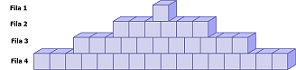
\includegraphics[width=0.45\textwidth]{../images/57c79607ac0a75446759bf7de89522cf0cbcea57}
    \caption{Ilustración de los bloques de plástico}
    \label{fig:bloques_plastico}
\end{figure}
